\documentclass[border=4pt]{standalone}
\usepackage{amsmath,amssymb,amsfonts}
\usepackage{xcolor,colortbl,array,booktabs,multirow}
\usepackage{tikz}
\usepackage{pgfplots}
\pgfplotsset{compat=1.16}
\usetikzlibrary{arrows, automata, backgrounds, calendar, chains, decorations,
    matrix, mindmap, patterns, petri, positioning, shadows, shapes.geometric,
    trees, shapes, decorations.pathreplacing, calc, tikzmark, arrows.meta,
    intersections, fit, graphs, quotes, angles, decorations.markings}
\newcommand{\st}{\text{ s.t. }}
\newcommand{\x}{\mathbf{x}}
\renewcommand{\b}{\mathbf{b}}
\renewcommand{\c}{\mathbf{c}}
\newcommand{\A}{\mathbf{A}}
\newcommand{\y}{\mathbf{y}}
\newcommand{\z}{\mathbf{z}}
\newcommand{\R}{\mathbb{R}}
\newcommand{\RR}{\mathbb{R}}
\newcommand{\Z}{\mathbb{Z}}
\newcommand{\ZZ}{\mathbb{Z}}
\newcommand{\npcomplete}{NP-complete}
\providecommand{\true}{\text{TRUE}}
\providecommand{\false}{\text{FALSE}}
\tikzset{vertex/.style={circle,fill=black!25,minimum size=20pt,inner sep=0pt},
    edge/.style={draw,thick,-},weight/.style={font=\small},
    selected vertex/.style={vertex, fill=red!24},
    selected edge/.style={draw,line width=2pt,-,red!50},
    ignored edge/.style={draw,line width=2pt,-,black!20}}
\newcommand{\vect}{\vec}
\providecommand{\ds}{\displaystyle}
\providecommand{\longvect}{\overrightarrow}
\usepackage[normalem]{ulem}
\definecolor{ocre}{RGB}{243,102,25}
\providecommand{\leftB}{\left[}
\providecommand{\rightB}{\right]}
\tikzset{directed/.style={postaction={decorate,decoration={markings,mark=at position .65 with {\arrow{>}}}}},
    directed1/.style={postaction={decorate,decoration={markings,mark=at position .65 with {\arrow{>}}}}}}
\begin{document}
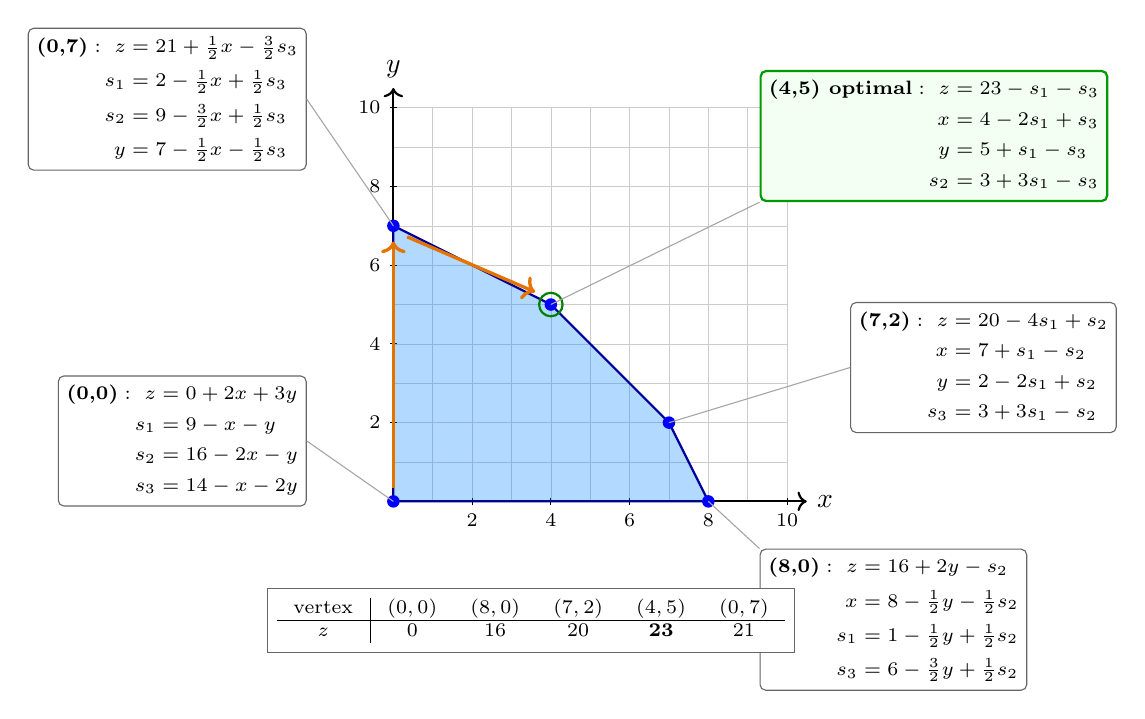
\begin{tikzpicture}[scale=0.5,
    dictbox/.style={draw=black!60, fill=white, rounded corners=2pt, inner sep=3pt, font=\scriptsize},
    optbox/.style={draw=green!60!black, thick, fill=green!5, rounded corners=2pt, inner sep=3pt, font=\scriptsize},
    connect/.style={black!35, thin}]
    % Grid and axes
    \draw[gray!40, very thin, step=1] (0,0) grid (10,10);
    \draw[->, thick] (0,0) -- (10.5,0) node[right] {$x$};
    \draw[->, thick] (0,0) -- (0,10.5) node[above] {$y$};
    \foreach \x in {2,4,6,8,10} \draw (\x,0.08) -- (\x,-0.08) node[below] {\scriptsize \x};
    \foreach \y in {2,4,6,8,10} \draw (0.08,\y) -- (-0.08,\y) node[left] {\scriptsize \y};

    % Feasible region: (0,0) -- (8,0) -- (7,2) -- (4,5) -- (0,7) -- cycle
    \fill[blue!50!cyan, opacity=0.3] (0,0) -- (8,0) -- (7,2) -- (4,5) -- (0,7) -- cycle;
    \draw[blue!60!black, thick] (0,0) -- (8,0) -- (7,2) -- (4,5) -- (0,7) -- cycle;

    % Simplex path taken in the text: (0,0) -> (0,7) -> (4,5)
    \draw[->, very thick, orange!90!black] (0,0.35) -- (0,6.6);
    \draw[->, very thick, orange!90!black] (0.35,6.72) -- (3.6,5.32);

    % Vertices
    \foreach \p in {(0,0),(8,0),(7,2),(4,5),(0,7)} \node[blue] at \p [circle,fill,inner sep=1.6pt]{};
    \node[green!50!black] at (4,5) [circle,draw,thick,inner sep=3pt]{};

    % Dictionary boxes
    \node[dictbox, anchor=north east] (d00) at (-2.2,3.2) {$\begin{aligned}[t]
        \textbf{(0,0)}:\ z &= 0 + 2x + 3y\\
        s_1 &= 9 - x - y\\
        s_2 &= 16 - 2x - y\\
        s_3 &= 14 - x - 2y
        \end{aligned}$};
    \node[dictbox, anchor=south east] (d07) at (-2.2,8.4) {$\begin{aligned}[t]
        \textbf{(0,7)}:\ z &= 21 + \tfrac12 x - \tfrac32 s_3\\
        s_1 &= 2 - \tfrac12 x + \tfrac12 s_3\\
        s_2 &= 9 - \tfrac32 x + \tfrac12 s_3\\
        y &= 7 - \tfrac12 x - \tfrac12 s_3
        \end{aligned}$};
    \node[optbox, anchor=south west] (d45) at (9.3,7.6) {$\begin{aligned}[t]
        \textbf{(4,5) optimal}:\ z &= 23 - s_1 - s_3\\
        x &= 4 - 2s_1 + s_3\\
        y &= 5 + s_1 - s_3\\
        s_2 &= 3 + 3s_1 - s_3
        \end{aligned}$};
    \node[dictbox, anchor=west] (d72) at (11.6,3.4) {$\begin{aligned}[t]
        \textbf{(7,2)}:\ z &= 20 - 4s_1 + s_2\\
        x &= 7 + s_1 - s_2\\
        y &= 2 - 2s_1 + s_2\\
        s_3 &= 3 + 3s_1 - s_2
        \end{aligned}$};
    \node[dictbox, anchor=north west] (d80) at (9.3,-1.2) {$\begin{aligned}[t]
        \textbf{(8,0)}:\ z &= 16 + 2y - s_2\\
        x &= 8 - \tfrac12 y - \tfrac12 s_2\\
        s_1 &= 1 - \tfrac12 y + \tfrac12 s_2\\
        s_3 &= 6 - \tfrac32 y + \tfrac12 s_2
        \end{aligned}$};

    % Connectors from boxes to vertices
    \draw[connect] (d00.east) -- (0,0);
    \draw[connect] (d07.east) -- (0,7);
    \draw[connect] (d45.south west) -- (4,5);
    \draw[connect] (d72.west) -- (7,2);
    \draw[connect] (d80.north west) -- (8,0);

    % Objective value table
    \node[draw=black!60, fill=white, anchor=north, font=\scriptsize] at (3.5,-2.2) {
        \begin{tabular}{c|ccccc}
        vertex & $(0,0)$ & $(8,0)$ & $(7,2)$ & $(4,5)$ & $(0,7)$\\
        \hline
        $z$ & $0$ & $16$ & $20$ & $\mathbf{23}$ & $21$
        \end{tabular}};
\end{tikzpicture}
\end{document}
